\section{Detailed One-Iteration Calculations}
\label{app:calculations}

\subsection{FDR: Complete Updates and Support Preservation}
Starting from an enabled state with integer $n,v,c$,
$1\leq v<n$ and $0\leq c<v$, a bit $\beta$ gives
$t=2c+\beta$ and $0\leq t<2v<2n$.
If $t<n$, the complete successor is $(2v,t)$ and satisfies
$0\leq t<\min(2v,n)$. If $t\geq n$, the successor is
$(2v-n,t-n)$; here $1\leq2v-n<n$ and
$0\leq t-n<2v-n$. Both cases preserve \eqref{eq:fdr-support}, and
initialization gives $(v,c)=(1,0)$ for every $n\geq1$.
The probability-weighted sum of these complete updates is exactly
\eqref{eq:fdr-post}. In both cases the updated difference is
\[
 v'-c'=2(v-c)-\beta.
\]
For $\beta=0$, a continuing outcome satisfies
\[
 n-v'+c'=n-v+c-(v-c)\leq n-v+c-1.
\]
A terminal outcome has guarded certificate zero. This proves the
affine descent used in \Cref{thm:fdr} over the entire supplied support,
not merely the states reachable for one fixed $n$.
The same difference identity also gives the logarithmic descent for
\eqref{eq:fdr-log-variant}.

\subsection{FDR: Shortest Paths and a Logarithmic Variant}
\label{app:fdr-log-variant}
The logarithmic variant used in the earlier FDR AST argument
\cite{zilken2026verifyingsamplingalgorithmsdistributional} also fits
the present rule. Keeping $I_{\mathrm{FDR}}$, $v$, and
$\varepsilon=1/2$ fixed, we may choose
\begin{equation}
 u_{\log}(\sigma)=
 \begin{cases}
 \left\lceil\log_2\!\left(\dfrac{n}{v-c}\right)\right\rceil,&v<n,\\
 0,&v\geq n.
 \end{cases}
 \label{eq:fdr-log-variant}
\end{equation}
For an enabled state, $1\leq v-c<n$, so the logarithm is positive
and finite; the ceiling makes $u_{\log}$ a positive integer.
This variant is motivated by the number of complete iterations needed
to reach a terminal state along a possible sequence of bits.
Write $d_{\min}(\sigma)$ for the shortest such number: a step from
an enabled state is one complete update $F_0$ or $F_1$, and the target
is any state with $v\geq n$. Terminal states have distance zero.

To see that a finite path to termination exists, put $\Delta=v-c$.
Every zero-bit iteration doubles $\Delta$, including iterations that
recycle. After
$k=\lceil\log_2(n/\Delta)\rceil$ consecutive zero bits, either the loop
has terminated or its difference would be $2^k\Delta\geq n$.
The latter is impossible at an enabled loop head, where
$\Delta\leq n-1$. This sequence therefore reaches a terminal state
within $k$ iterations and has probability at least $2^{-k}>0$. Hence
\begin{equation}
 d_{\min}(\sigma)\leq u_{\log}(\sigma).
 \label{eq:fdr-shortest-distance-bound}
\end{equation}
The bound need not be exact. For $n=6$ and $(v,c)=(4,2)$, it gives
$u_{\log}=2$, but both successors $(8,4)$ and $(8,5)$ are terminal,
so $d_{\min}=1$. \Cref{fig:fdr-iteration-variants} compares the
logarithmic variant $u_{\log}$ with the exact distance $d_{\min}$.

The zero-bit outcome proves descent of $u_{\log}$ directly: if it
continues, then
\[
 u_{\log}(F_0(\sigma))
 =\left\lceil\log_2\!\left(\frac{n}{2(v-c)}\right)\right\rceil
 =u_{\log}(\sigma)-1;
\]
if it terminates, its value is zero. On enabled states with
$v(\sigma)\leq r$, we have $n\leq r$ and therefore
$u_{\log}\leq\lceil\log_2 n\rceil\leq\lceil\log_2 r\rceil$.
For $r<1$, the sublevel contains only terminal states.
Thus $u_{\log}$ satisfies the same rule.
The distance $d_{\min}$ is another valid variant: the first bit of
a shortest path decreases it by one with probability at least $1/2$,
and \eqref{eq:fdr-shortest-distance-bound} supplies its sublevel bound.
The affine variant avoids both a logarithm and a shortest-path
calculation, which is why we use it for the main proof.

% This new drawing contracts all recycling updates and shows actual
% shortest distances alongside the terminal-normalized logarithmic variant.
\begin{figure}[t]
 \centering
 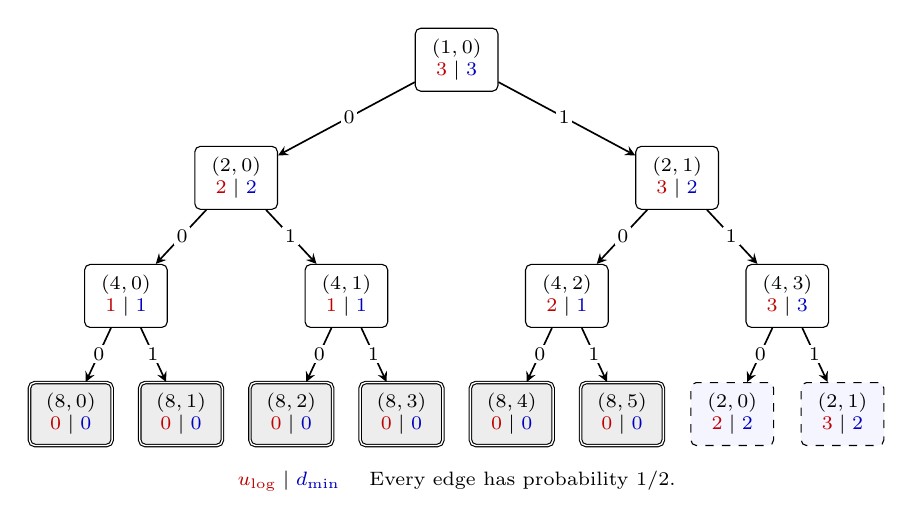
\begin{tikzpicture}[
   x=1.4cm,y=1cm,>=stealth,
   fdrstate/.style={draw,rounded corners=2pt,minimum width=10.5mm,
     minimum height=8mm,inner sep=2pt,align=center,font=\scriptsize},
   fdrterminal/.style={fdrstate,fill=black!7,double,double distance=0.5pt},
   fdrrecycled/.style={fdrstate,dashed,fill=blue!4},
   fdrbit/.style={font=\scriptsize,fill=white,inner sep=1pt},
   fdredge/.style={->,semithick}
 ]
 % Each node displays (v,c), then u_log | d_min.
 \node[fdrstate] (s10) at (3.5,4.5)
   {$(1,0)$\\$\textcolor{red!75!black}{3}\mid\textcolor{blue!75!black}{3}$};
 \node[fdrstate] (s20) at (1.5,3)
   {$(2,0)$\\$\textcolor{red!75!black}{2}\mid\textcolor{blue!75!black}{2}$};
 \node[fdrstate] (s21) at (5.5,3)
   {$(2,1)$\\$\textcolor{red!75!black}{3}\mid\textcolor{blue!75!black}{2}$};
 \node[fdrstate] (s40) at (0.5,1.5)
   {$(4,0)$\\$\textcolor{red!75!black}{1}\mid\textcolor{blue!75!black}{1}$};
 \node[fdrstate] (s41) at (2.5,1.5)
   {$(4,1)$\\$\textcolor{red!75!black}{1}\mid\textcolor{blue!75!black}{1}$};
 \node[fdrstate] (s42) at (4.5,1.5)
   {$(4,2)$\\$\textcolor{red!75!black}{2}\mid\textcolor{blue!75!black}{1}$};
 \node[fdrstate] (s43) at (6.5,1.5)
   {$(4,3)$\\$\textcolor{red!75!black}{3}\mid\textcolor{blue!75!black}{3}$};
 \foreach \j in {0,...,5} {
   \node[fdrterminal] (t\j) at (\j,0)
     {$(8,\j)$\\$\textcolor{red!75!black}{0}\mid\textcolor{blue!75!black}{0}$};
 }
 \node[fdrrecycled] (r20) at (6,0)
   {$(2,0)$\\$\textcolor{red!75!black}{2}\mid\textcolor{blue!75!black}{2}$};
 \node[fdrrecycled] (r21) at (7,0)
   {$(2,1)$\\$\textcolor{red!75!black}{3}\mid\textcolor{blue!75!black}{2}$};
 \foreach \from/\to/\bit in {
   s10/s20/0,s10/s21/1,
   s20/s40/0,s20/s41/1,s21/s42/0,s21/s43/1,
   s40/t0/0,s40/t1/1,s41/t2/0,s41/t3/1,
   s42/t4/0,s42/t5/1,s43/r20/0,s43/r21/1} {
   \draw[fdredge] (\from) -- node[fdrbit,pos=0.48] {$\bit$} (\to);
 }
 \node[font=\scriptsize,align=center] at (3.5,-0.85)
   {$\textcolor{red!75!black}{u_{\log}}\mid\textcolor{blue!75!black}{d_{\min}}$
    \quad Every edge has probability $1/2$.};
 \end{tikzpicture}
 \caption{Three-iteration unfolding of FDR for $n=6$. Each node gives
 $(v,c)$ and, below it, the logarithmic variant $u_{\log}$ (red, left) and the
 shortest distance $d_{\min}$ (blue, right). Edge labels are sampled bits.
 Double borders mark terminal states, where both functions are zero.
 Dashed leaves repeat earlier states after recycling; they are not
 terminal. Each edge includes all updates of one loop iteration.}
 \label{fig:fdr-iteration-variants}
\end{figure}

\subsection{FLDR: The Exact Tree Contract}
Put $w_i=a_i$ for $1\leq i\leq n$ and $w_{n+1}=2^k-m$, so
$\sum_iw_i=2^k$. For $0\leq c\leq k$, let $e_{i,c}\in\{0,1\}$ be
the bit of $w_i$ in position $k-c$, and put $h_c=\sum_i e_{i,c}$.
At depth zero there is one node. Designate $h_0$ nodes as leaves and
put $q_0=1-h_0$. At each subsequent depth $c$, expand the $q_{c-1}$
internal nodes, producing $2q_{c-1}$ nodes, and designate $h_c$ of
them as leaves. Thus
\[
 q_c=2q_{c-1}-h_c
     =2^c-\sum_{i=1}^{n+1}
         \left\lfloor\frac{w_i}{2^{k-c}}\right\rfloor
     =\sum_{i=1}^{n+1}
         \left\{\frac{w_i}{2^{k-c}}\right\},
\]
where braces denote fractional part. Consequently $q_c$ is a
nonnegative integer at most $n$, and $q_k=0$. In particular, the
construction always has enough nodes for its designated leaves and
has no internal node at depth $k$.

Set $\phi_h(c)=q_c$. In every row place the internal nodes first and
then one leaf labeled $i$ for each $e_{i,c}=1$, in decreasing label
order. At positive depth the row has $2q_{c-1}\leq2n$ nodes.
An internal node with index $d<q_c$ therefore has the two valid children
$2d,2d+1$ in the next row. Give internal nodes label zero in $H$.
A root leaf occurs precisely when a single positive weight equals
$2^k$; it is accepting, since $w_{n+1}<2^k$.
These observations justify the support predicate in
\Cref{sec:fldr}, including $d<2n$ and the absence of enabled states at
depth $k$. A tighter bound $d\leq n$ would be false: for weights
$(4,5)$, the accepting node $(c,d)=(2,3)$ is reachable although $n=2$.

Each row has at most one leaf with label $n+1$. Hence among the two
children of any internal node at least one avoids rejection. A rejecting
child resets to the root, which is internal whenever a rejecting leaf
exists. A non-rejecting child either accepts or remains internal at
depth $c+1$. Thus the post-distribution has non-reset mass at least
$1/2$, and every such outcome strictly decreases the guarded function
$k-c$. This is the structural contract used by the abstract synthesis
instance. It follows from the construction for all positive integer
weight vectors; finite checks of generated trees are additional tests,
not a replacement for this argument.

For completeness, the leaf construction also preserves the proposal
probabilities. A leaf labeled $i$ at depth $c$ has probability $2^{-c}$,
so one traversal returns $i$ with probability
$\sum_c e_{i,c}2^{-c}=w_i/2^k$. Rejection restarts from the root.
Writing $p_i$ for the eventual probability of outcome $i$, first-traversal
conditioning gives
\[
 p_i=\frac{a_i}{2^k}+\frac{2^k-m}{2^k}p_i,
 \qquad\text{hence}\qquad p_i=\frac{a_i}{m}.
\]
The AST proof ensures that these probabilities account for the entire
output mass. This direct argument also confirms that reordering leaves
within a row does not alter the sampled distribution.

\subsection{Han--Hoshi: Boundary Counting and a Tail Bound}
\label{app:han-hoshi-tail}
For a nonempty interval $J\subseteq[0,1)$, containment in a target
interval is equivalent to having no internal target boundary strictly
inside $J$. An endpoint coinciding with a target boundary creates no
ambiguity because all intervals are half-open. Splitting $J$ into its
two half-open children assigns each interior target boundary to at most
one child, proving \eqref{eq:han-hoshi-boundary-split}.

Let $\sigma_t$ be the state after $t$ sampling-loop iterations, with
terminal states held fixed, and put $\mathsf V_t=\mathsf V(\sigma_t)$
for the certificate from \Cref{sec:HanHoshi}. Write
$T=\inf\{t\in\mathbb N\mid\sigma_t(r)\ne0\}$, with
$\inf\varnothing=\infty$, for the number of iterations until termination.
The one-step estimate proved there is
$\mathbb E[\mathsf V_{t+1}\mid\sigma_t]\leq\mathsf V_t/2$.
This remains true in the exceptional enabled
case with no interior boundary: both children terminate. Starting from
$J(0,1)$, one has $\mathsf V_0=\max\{1,n-1\}$, and induction yields
\[
 \Pr(T>t)\leq\mathbb E[\mathsf V_t]
 \leq 2^{-t}\max\{1,n-1\},\qquad t\in\mathbb N.
\]
Here $[T>t]\leq\mathsf V_t$ because every enabled state has value at least
one. This bound proves AST independently and even gives a finite
expected number of bits for each finite weight vector. The main text
uses the two-certificate rule to expose the common proof interface
across the examples; this example does not require the full strength
of that rule.
